\documentclass[10pt,twocolumn,letterpaper]{article}

\usepackage{cvpr}
\usepackage{times}
\usepackage{epsfig}
\usepackage{graphicx}
\usepackage{amsmath}
\usepackage{amssymb}
\usepackage[utf8]{inputenc}
\usepackage{booktabs,tabularx,enumitem,ragged2e}

% Include other packages here, before hyperref.

% If you comment hyperref and then uncomment it, you should delete
% egpaper.aux before re-running latex.  (Or just hit 'q' on the first latex
% run, let it finish, and you should be clear).
\usepackage[breaklinks=true,bookmarks=false]{hyperref}

\cvprfinalcopy % *** Uncomment this line for the final submission

\def\cvprPaperID{****} % *** Enter the CVPR Paper ID here
\def\httilde{\mbox{\tt\raisebox{-.5ex}{\symbol{126}}}}

% Pages are numbered in submission mode, and unnumbered in camera-ready
%\ifcvprfinal\pagestyle{empty}\fi
\setcounter{page}{1}
\begin{document}

%%%%%%%%% TITLE
\title{Project Report: Scan2Cap}

\author{Felix Wimbauer\\
Technical University of Munich\\
{\tt\small felix.wimbauer@tum.de}
% For a paper whose authors are all at the same institution,
% omit the following lines up until the closing ``}''.
% Additional authors and addresses can be added with ``\and'',
% just like the second author.
% To save space, use either the email address or home page, not both
\and
Nicolas Seppich\\
Technical University of Munich\\
{\tt\small nicolas.seppich@tum.De}
\and

\small
Supervisor: Dave Zhenyu Chen\\
\small
Technical University of Munich\\
{\tt\small zhenyu.chen@tum.de }
}

\maketitle
%\thispagestyle{empty}

%%%%%%%%% ABSTRACT
\begin{abstract}
In this work, we aim to investigate the task of generating a description for a target object in context to its environment in the 3D domain. To this end, we propose a pipeline which combines concepts from 3D object detection and visal attention-based captioning. The proposed pipeline first uses VoteNet to extract feature vectors of the scene. It then combines this information with the features of the object of interest, which are extracted by PointNet++, and feeds this data into an LSTM captioning mechanism, that generates a caption of the object in context of the scene.  
   
\end{abstract}

%%%%%%%%% BODY TEXT
\section{Introduction}

Extracting a detailed and semantic correct understanding of the layout of a 3D scene is crucial for many tasks, e.g. in robotics for navigation and interaction with objects. This includes relating the 3D positions of the objects and their spatial extent, so that a semantically correct description of the objects' environment is generated.
However, to the best of our knowledge, there has been no work so far to generate a description of an object representation in point clouds or 3D data.

Therefore, we are interested in implementing a pipeline to obtain a description for a given object in a 3D scan, using state-of-the-art point cloud feature extractors, object detectors, and a captioning mechanism to generate a semantic description for a given object in the 3D scene. This allows the object to be placed in a global semantic context within its environment.
 
%-------------------------------------------------------------------------
\section{Related Work}
Our work will be based on the ScanRefer dataset \cite{chen2019scanrefer}. This dataset consists of 1513 RGB-D scans of ScanNet \cite{dai2017scannet} and contains approximately 5 unique object descriptions for each object in each scene. The work of \cite{chen2019scanrefer} will also be used as guideline in this project.

The extraction of features on point clouds is presented by \cite{qi2017pointnet++}, who apply the feature extraction directly on the point cloud on a hierarchical level, allowing the extraction of local features in a global context. 
The task of object detection on point clouds is studied by \cite{qi2019deep}. 

Methods for image captioning using visual attention are described by \cite{xu2015show}, \cite{lu2017knowing} and \cite{anderson2018bottom}.
These methods have in common, that they generate a caption for the entire image.
Since our goal includes using a bounding box for the object to be set in context to the scene, the work of \cite{rohrbach2016grounding} is also of interest for this project. 

%-------------------------------------------------------------------------
\section{Architecture}

Given a point cloud $\mathit{p \in R^{N\times(d+C)}}$ and an object in that scene, which is described by a target bounding box $b_{target}\in R^6$, our goal is to generate a meaningful caption for the object embedded in the context of the scene. To this end, we used three different pipelines, which are described in the following.

\subsection{Baseline}

To extract information from the point cloud, we use a PointNet++ \cite{qi2017pointnet++} model. To give the network information about which object we are interested in, we add a new feature channel to each point that masks all points that lay within the bounding box of the object. To ensure that we receive meaningful features, we use weights pretrained for classification of the masked object. The idea behind this is that classification will not only use information from the masked objects, but also global features, for example from close-by objects. 

To generate the caption, we use a classical LSTM with an appended fully-connected layer. The fully-connected layer acts as a word classifier and maps the hidden state $h_{t}$ of the LSTM to our vocabulary. As input, the LSTM receives the feature vector extracted from the point cloud and the word embedding vector of the previously generated word. The word embedding is taken from a pre-computed GloVe \cite{pennington2014glove} word embedding matrix. This structure of the iterative caption generation is similar to \cite{xu2015show}.

\subsection{Better Feature Extraction with VoteNet}

Because PointNet++ is pretrained to classify the object of interest there is no guarantee that the feature vector will give high-quality information about the global context, thus limiting the baseline approach. In the second architecture iteration, we therefore employ a VoteNet \cite{qi2019deep} network, which computes a fixed number of object proposals and according feature vectors for our point cloud. Those feature vectors nicely describe the context of our scan and help the network to understand the surroundings of the object we want to describe. Because the number of proposals may vary and the proposals are not in a fixed order, we average pool them to obtain a concise representation of the information. This pooled feature vector is finally concatenated with the feature vector from PointNet++ and the embedding vector of the previously predicted word to then be passed into the LSTM.

\subsection{Better Captioning with Attention}

Average pooling the feature vectors from VoteNet is not ideal as often only a small number of the object proposals is relevant for the final caption. Therefore, in the third model iteration we replace the average pooling step from before with an attention mechanism, as it is described in \cite{xu2015show}. The attention mechanism receives the hidden state of the captioning LSTM from the previous iteration and the feature vectors of the object proposals. It then uses a series of fully-connected layers to predict relevancy scores for the different object proposals that are turned into probabilities using the softmax function. Instead of average pooling, we can now multiply all feature vectors with their respective probability and sum over all of them. This approach allows our model to select the most relevant object for each token in the caption and make word predictions that better match the the context of the scene.

\autoref{fig:pipeline} summarizes the project pipeline.

%\begin{figure*}
%	\centering
%	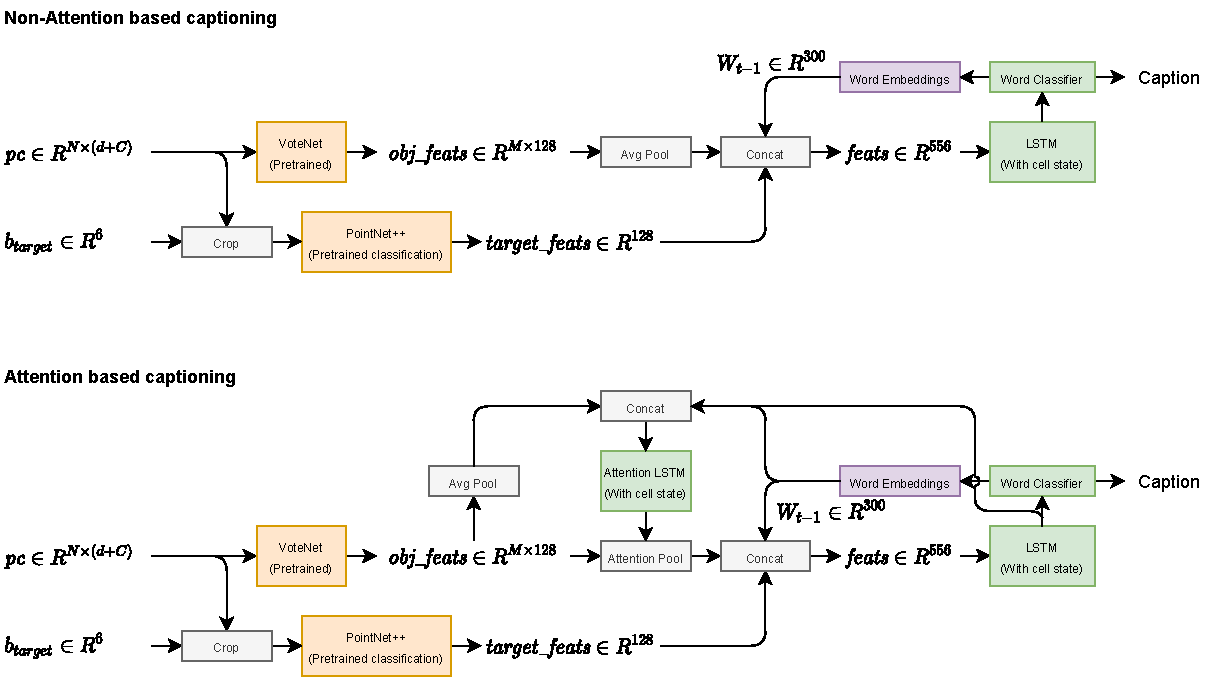
\includegraphics[width=\textwidth]{figures/pipeline_sketch.pdf}
%	\caption{Pipeline for project}
%	\label{fig:pipeline}
%\end{figure*}

\begin{table*}
	\centering
	\begin{tabularx}{\textwidth}{l|l}
	\textbf{Date} & \textbf{Milestones} \\
	\hline
	\textbf{First Presentation} & 
	\begin{minipage}[t]{\textwidth}
		\begin{itemize}[nosep, wide=0pt, leftmargin=*, after=\strut]
			\item Get familiar with dataset
			\item Test different sub components of pipeline (e.g. PointNet++, VoteNet and captioning mechanism)
			\item Start implementing the pipeline
			\item Optional: first training
		\end{itemize}  
	\end{minipage}\\
	\hline
	\textbf{Second Presentation} & 
	\begin{minipage}[t]{\linewidth}
		\begin{itemize}[nosep, wide=0pt, leftmargin=*, after=\strut]
			\item Finish implementation of pipeline
			\item Training and hyperparameter tuning
			\item Set up concept for attention mechanism
			\item Optional: start implementing attention
		\end{itemize}  
	\end{minipage}\\
	\hline
	\textbf{Final Presentation} & 
	\begin{minipage}[t]{\linewidth}
		\begin{itemize}[nosep, wide=0pt, leftmargin=*, after=\strut]
			\item Final results
			\item Optional: attention mechanism
		\end{itemize}  
	\end{minipage}\\
	\end{tabularx}
	\caption{Project milestones}
	\label{tab:milestones}
\end{table*}

{\small
\bibliographystyle{ieee_fullname}
\bibliography{report}
}

\end{document}
